\section{Motivation}
\frame{\tableofcontents[currentsection]}

% Omit these slides for now for time-purposes
\if 0
% Simple workflow
\begin{frame}{Motivation: Workflow}
\begin{figure}
\centering

\includegraphics[width=\textwidth]{figures/motivation-1.png}
\end{figure}
\end{frame}
\note[itemize]{%
\item Statisticians and clinicians come up with a new design.
\item Publish in a journal.
\item Takes time, but will get published eventually.
\item Convince pharma to use the new design.
\item Pharma then runs the trial.
}

\begin{frame}{Motivation: Workflow}
\begin{figure}
\centering
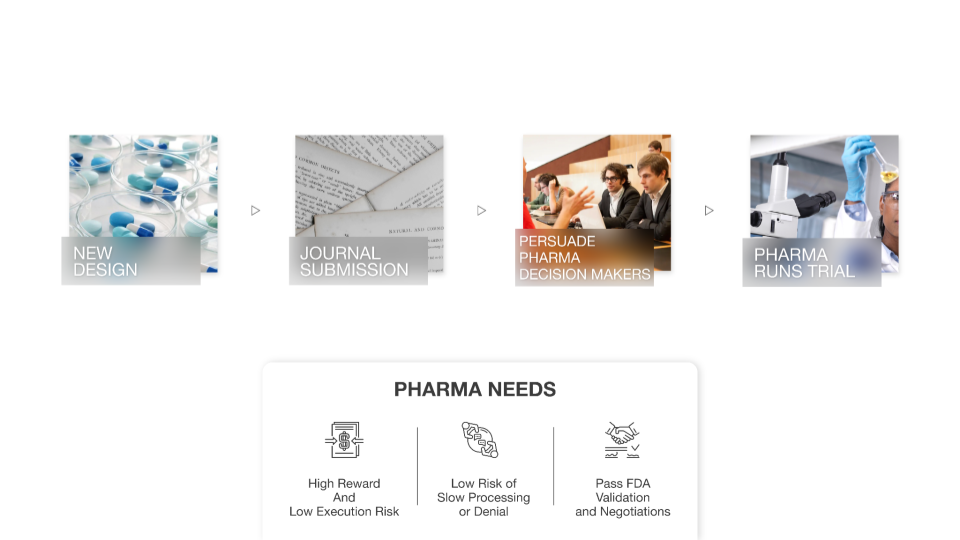
\includegraphics[width=\textwidth]{figures/motivation-2.png}
\end{figure}
\end{frame}
\note[itemize]{%
\item How do we convince pharma?
\item Make the case that the new design gives benefits that are worth the operating risks and the costs of complexity, which are, admittedly, much larger than one might expect.
\item If you can do that, that’s enough for your early phase trial! 
}

\begin{frame}{Motivation: Workflow}
\begin{figure}
\centering
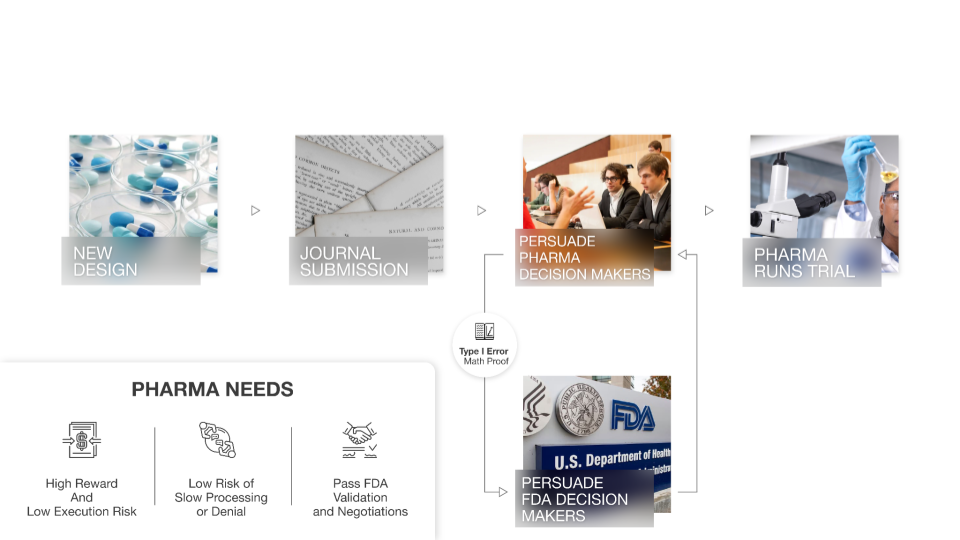
\includegraphics[width=\textwidth]{figures/motivation-3.png}
\end{figure}
\end{frame}
\note[itemize]{%
\item In late phases, need to convince pharma that the design is not going to affect their FDA processing.
\item In practice, the FDA has to be persuaded about wanting to use a new design.
\item A big factor in this process is showing control of Type I Error!
\item You might notice that we now have a circular dependency here, 
    because in order to get into FDA negotiations over a very niche design, 
    you need to have a sponsored application!
\item Hinders innovation.
}

\begin{frame}{Motivation: Workflow}
\begin{figure}
\centering
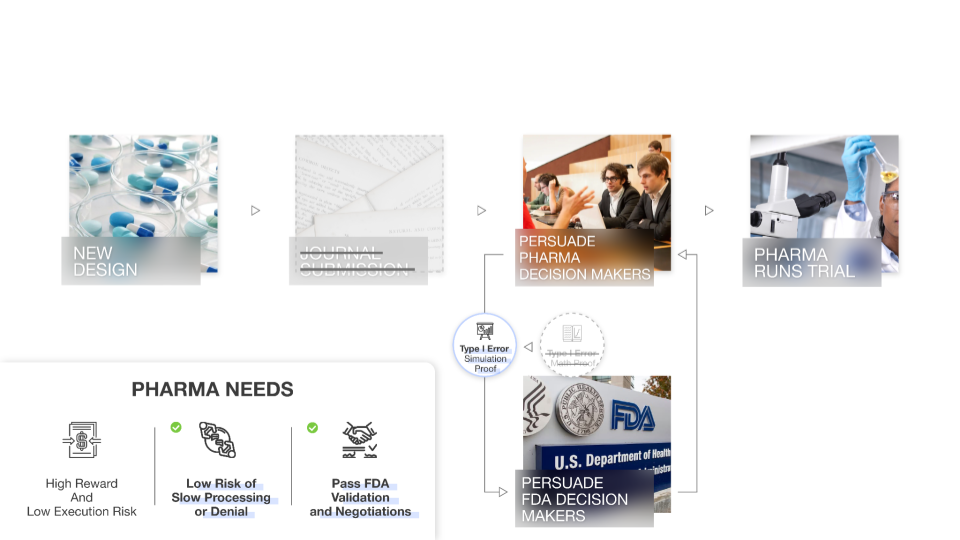
\includegraphics[width=\textwidth]{figures/motivation-4.png}
\end{figure}
\end{frame}
\note[itemize]{%
\item The key tool here is simulation!
\item Introduce a rigorous technique of ``proof by simulation''.
\item If pharma + FDA can agree on this technique, we can:
\item Iterate much more quickly.
\item Slice out the math for a Type I Error (math) proof
\item Slice out the need for journal validation.
\item And this is a wonderful thing! But, as a part of the trade-off, we get new questions and areas for negotiation which need to be settled in this key part of the innovation loop.
}
\fi

\begin{frame}{Our Goals}
\begin{itemize}
    \item Make the innovation process of trial designs \textbf{predictable} and \textbf{fast}!
    \item New technique: ``proof by simulation''.
    \item Proof of Type I Error control not just on simulated points in the null space, but also \emph{on the whole null space}.
    \item Enables:
    \begin{itemize}
        \item Automation of Type I Error mathematical proofs.
        \item Rigorous grounding for wide classes of complex designs
        \item Fast design and re-design iterations.
    \end{itemize}
\end{itemize}
\end{frame}

\begin{frame}{Simulation Challenges}
\begin{itemize}
    \item Some challenges raised by FDA at the start of the Complex Innovative Design (CID) Pilot Program:
    \begin{itemize}
        \item \textbf{How many points in the null hypothesis space to simulate?}
        \item \textbf{What is the computational complexity? Does it scale with multiple hypothesis testing?}
    \end{itemize}
    \item Other challenges:
    \begin{itemize}
        \item Simulation on a finite number of points
        in the null hypothesis space does not give guarantees for the whole space. 
        \textbf{How do we deal with composite nulls?}
        \item Simulation has Monte Carlo error. 
        \textbf{How do we control
        Type I Error (on the whole space) 
        accounting for the stochastic error?}
    \end{itemize}
\end{itemize}
\end{frame}
